\chapter{Results}
\label{sec:results}

This chapter presents the relevant results of the investigation and experimentation phases.
Presenting the tested cloud container orchestration platforms first,
followed by the results per evaluation requirement thereafter.

\section{Viable Solutions}
The following platforms were evaluated as potential solutions:
\begin{itemize}
  \item AWS Lambda (representing \textit{Serverless Functions})
  \item AWS ECS (representing \textit{Cloud Native})
        \begin{itemize}
          \item running on EC2 (representing \textit{Virtual Machines})
          \item running on Fargate (representing \textit{Serverless Containers})
        \end{itemize}
  \item AWS EKS (representing \textit{Kubernetes})
        \begin{itemize}
          \item running on EC2 (representing \textit{Virtual Machines})
          \item running on Fargate (representing \textit{Serverless Containers})
        \end{itemize}
\end{itemize}

\section{Experimentation Results}

\subsection{Performance and Latency}
Each platform was subjected to an identical set of broad benchmarks aiming to fully test the impact of both
selection of \emph{orchestration platform} and \emph{underlying architecture} in relation to performance.

\subsubsection{CPU}
\begin{figure}[htbp]
  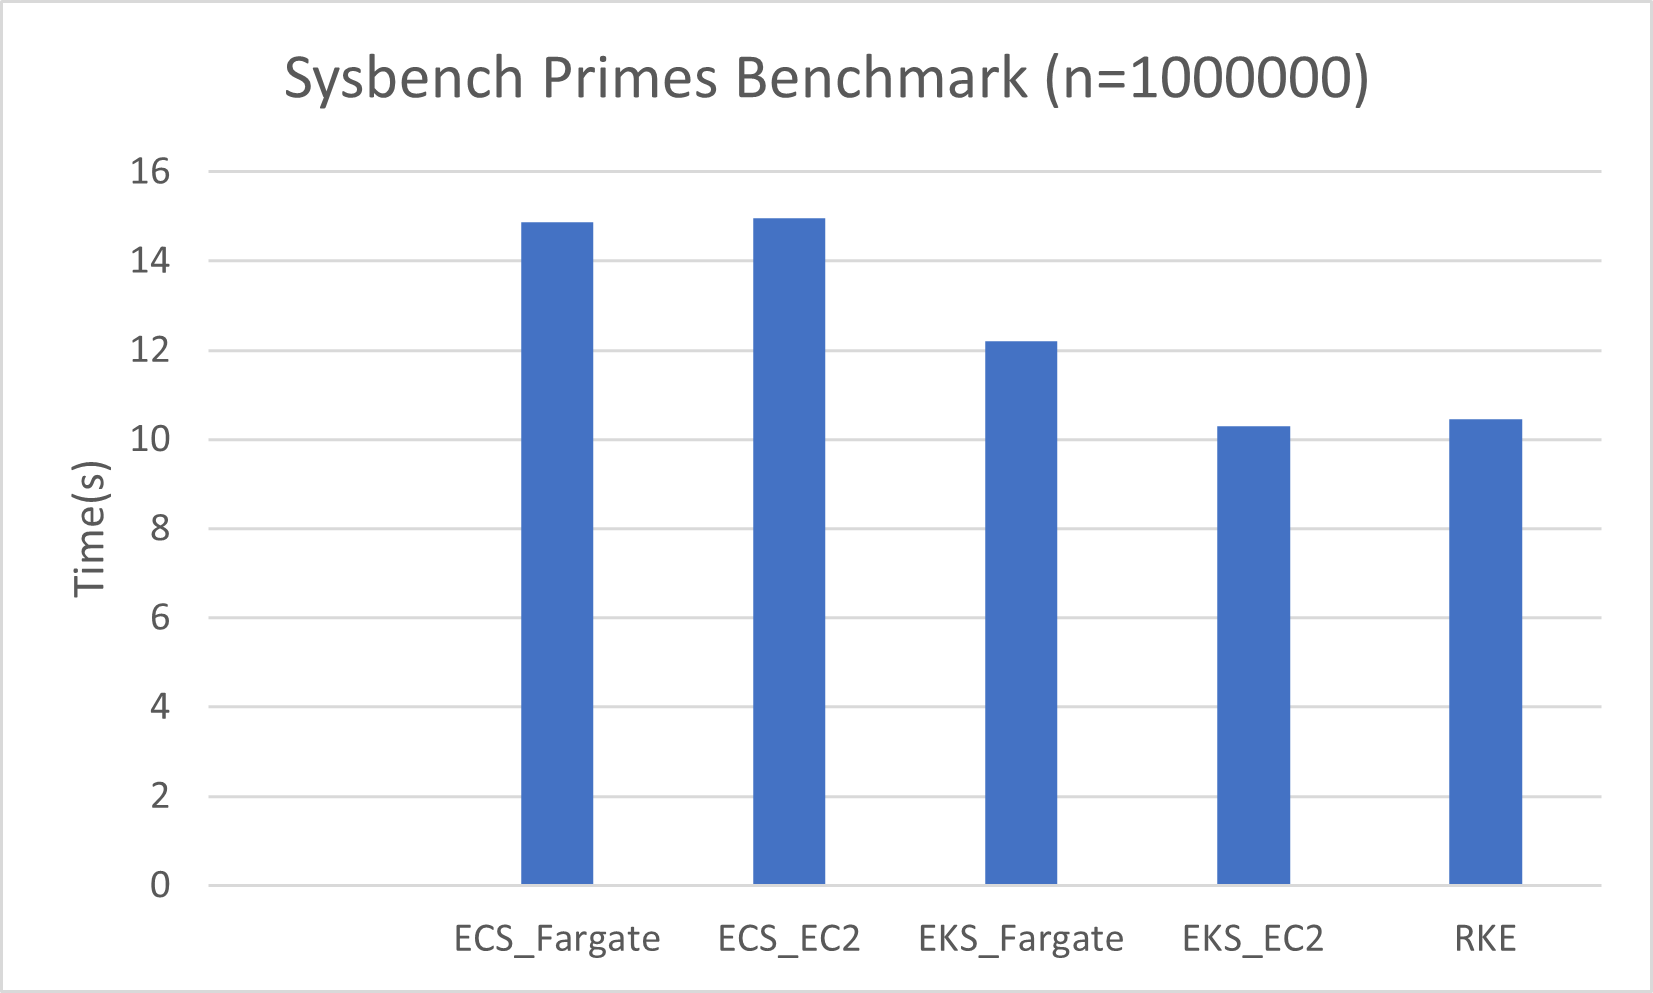
\includegraphics[width=\textwidth]{images/perf-sysbench.png}
  \caption{\emph{Performance}: Average time taken to compute primes up to 1000000 --- lower is better }
  \label{fig:perf_sysbench}
\end{figure}

\begin{figure}[htbp]
  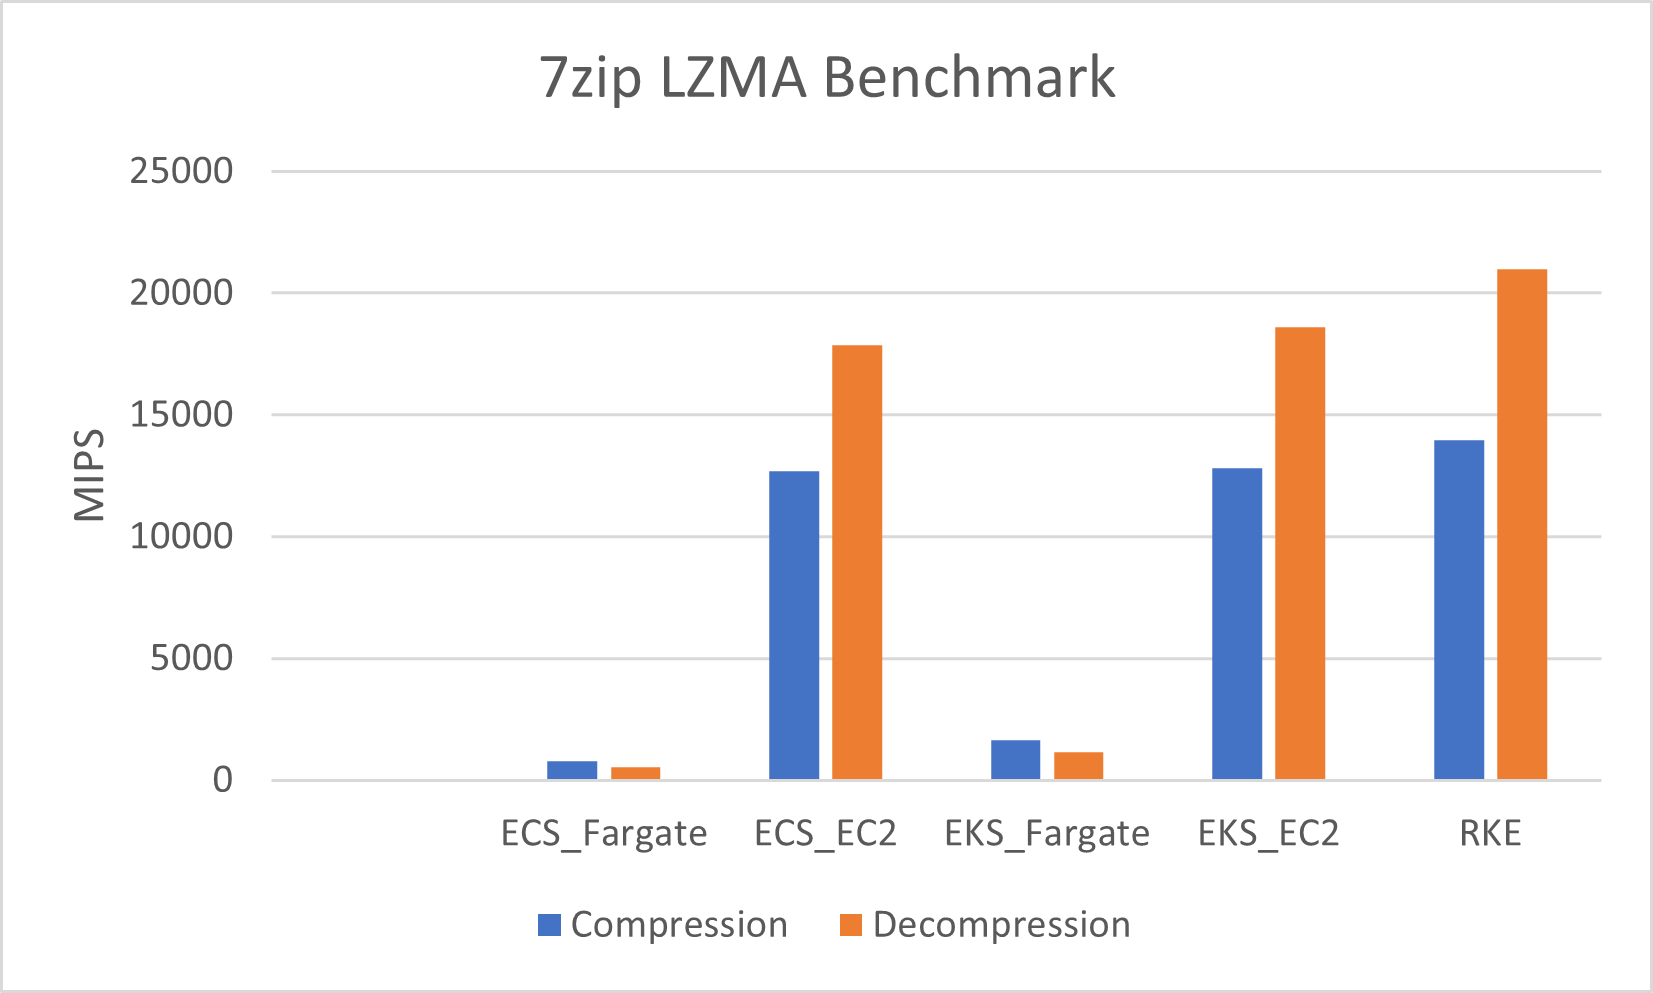
\includegraphics[width=\textwidth]{images/perf-7zip.png}
  \caption{\emph{Performance}: Average rating in MIPS to complete the 7zip LZMA Benchmark --- higher is better}
  \label{fig:perf_7zip}
\end{figure}

CPU performance was evaluated by performing CPU intensive tasks, such as computing prime numbers using a prime sieve,
and archive compression/ decompression and measuring the time taken to complete the respective tasks.

Figure \ref{fig:perf_sysbench} illustrates the amount of time taken (s) to compute primes up to 1000000 across 4 threads using \textit{Sysbench}.
The \textit{EC2} instance of the \textit{EKS} cluster outperformed the baseline \textit{RKE} instance by a margin of ~2\%,
with the \textit{fargate} solution performing 20 \% slower than the baseline.
Finally, both the \textit{ECS} backed instances completed the task about 50\% slower than the baseline. 

Figure \ref{fig:perf_7zip} illustrates the rating in million of instructions per second (MIPS) when performing the 7zip \textit{LZMA} compression and decompression benchmark.
Under this benchmark, the baseline \textit{RKE} instance posted the best result, with the two \textit{EC2} backed instances completing around 9\% (\textit{EKS}) and 10 \% (\textit{ECS}) less instructions respectively.
The two \textit{fargate} backed instances struggled immensely to complete this benchmark,
with the \textit{EKS} instance completing 80\% less tasks, and the \textit{ECS} instance completing 95 \% less tasks.

\noindent \newline It should be noted that due to runtime, and execution time-limit, limitations \textit{Lambda} did not complete in these CPU specific benchmarks.

\subsubsection{Memory}
Two criterion of memory performance was evaluated, the first being \emph{speed},
which was evaluated using the RAMSpeed, and \emph{bandwidth} using the MBW tool.

RAMSpeed performs four distinct memory intensive tasks with results, each measuring a different aspect of memory performance.
All results are recorded as a measurement of speed (MB/S).

This discussion will focus on last column in Figure \ref{fig:perf_RAMSpeed} as it illustrates the average speed recorded for the entirety of the benchmark (that is all four distinct tasks),
as the results (and performance difference) found in this table is wholly illustrative to the results found in each of the sub-tasks.
The \textit{EC2} backed \textit{EKS} instance outperformed the baseline \textit{RKE} instance by completing the tasks close to 36\% quicker.
This was followed by a significantly slower \textit{fargate} backed instance of \textit{EKS}, and \textit{EC2} backed \textit{ECS} instance,
which both completed close to 80\% slower than the baseline.
Finally the \textit{fargate} backed \textit{ECS} instance completed the benchmark close to 88\% slower.

\begin{figure}[htbp]
  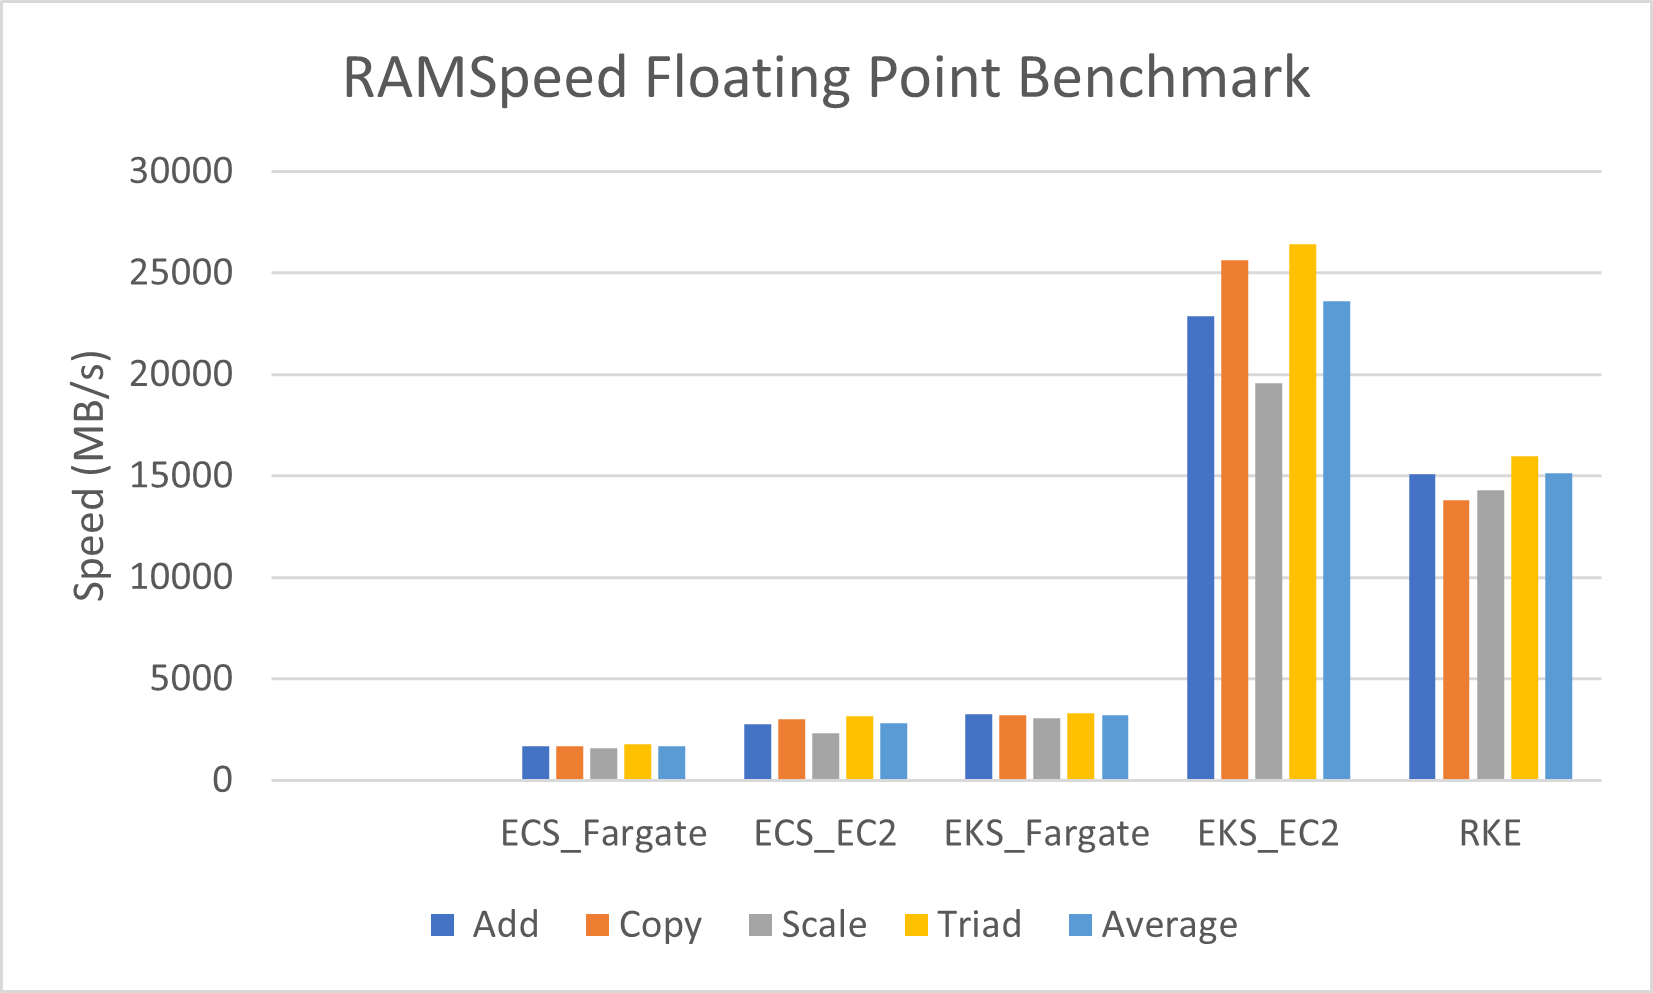
\includegraphics[width=\textwidth]{images/perf-RAMSpeed.png}
  \caption{\emph{Performance}: Average maximum speed achieved whilst completing the RAMSpeed Benchmark --- higher is better}
  \label{fig:perf_RAMSpeed}
\end{figure}

\begin{figure}[htbp]
  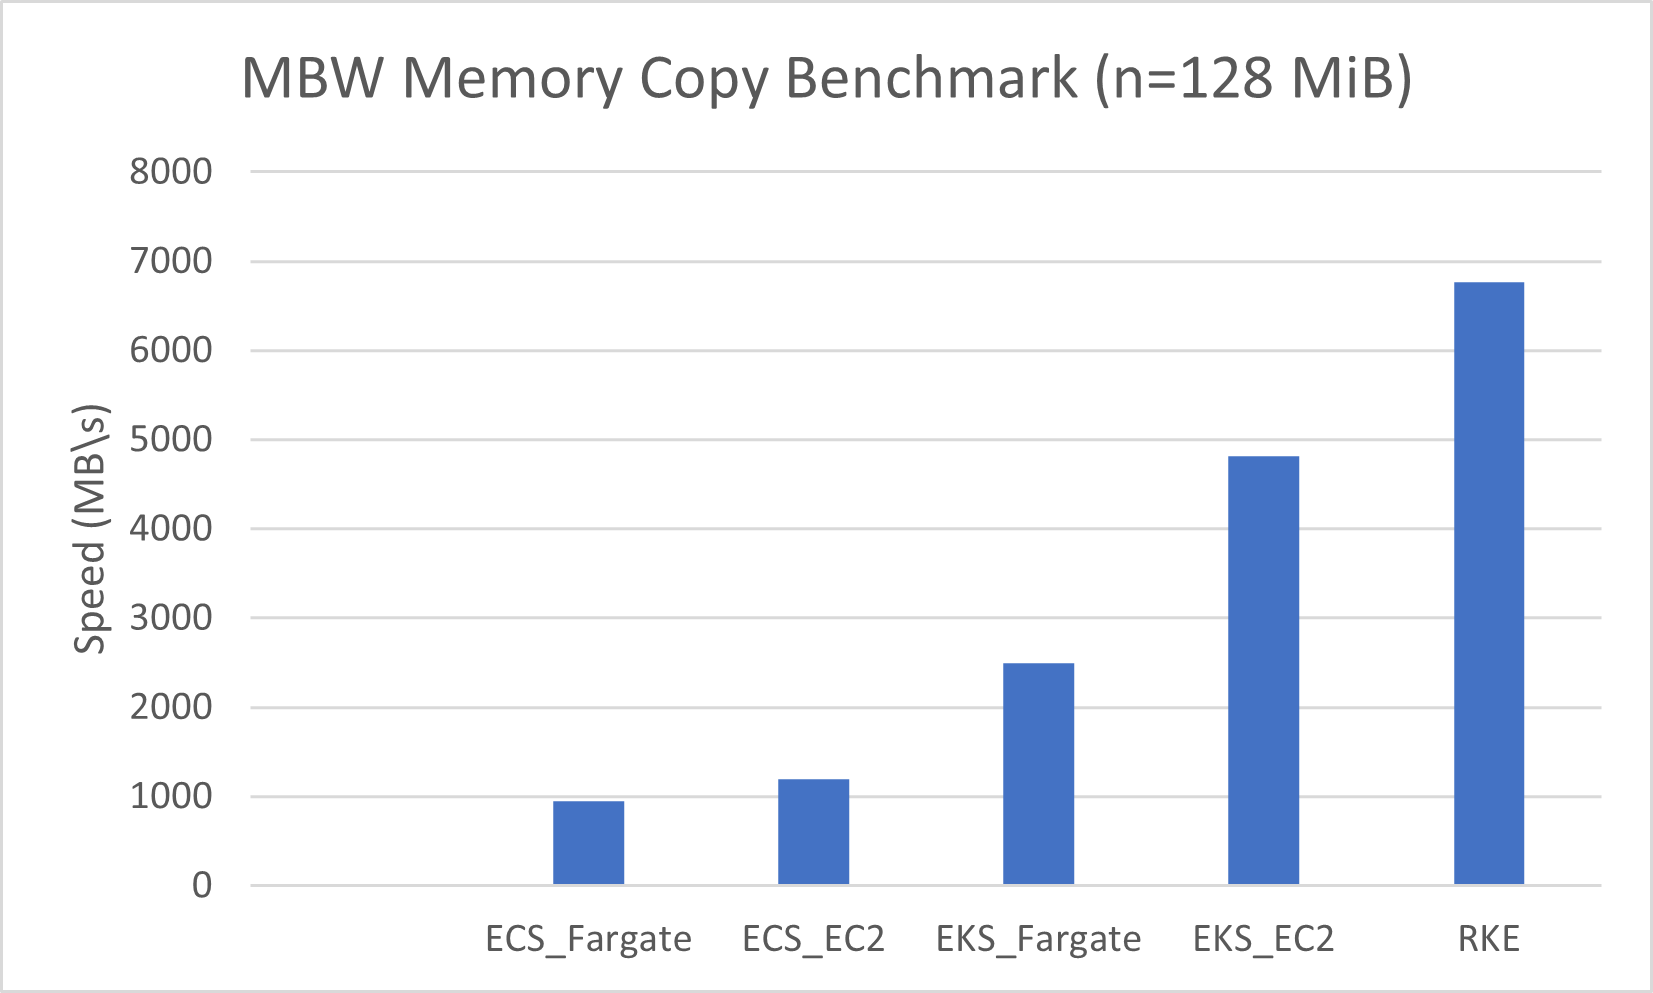
\includegraphics[width=\textwidth]{images/perf-MBW.png}
  \caption{\emph{Performance}: Average maximum speed achieved whilst completing the Memory Bandwidth Benchmark --- higher is better}
  \label{fig:perf_MBW}
\end{figure}

\noindent \newline MBW measures the amount of copy memory bandwidth available to a user-application in terms of speed (MB/s).

Figure \ref{fig:perf_MBW} illustrates the baseline \textit{RKE} instance completed this benchmark with the fastest speed, with the \textit{EC2} backed \textit{EKS} instance following at 29\% slower.
The \textit{fargate} backed \textit{EKS} instance completed 64\% slower,
followed by the two \textit{ECS} workloads at 83\% and 87\% slower for the \textit{EC2} and \textit{fargate} instances respectively.

\noindent \newline It should be noted that due to runtime, and execution time-limit, limitations \textit{Lambda} did not complete in these Memory specific benchmarks.

\subsubsection{I/O}
fs\_mark evaluates a system's underlying file-system by performing heavily synchronous IO tasks across multiple folders/drives, measured in terms of speed (number of files per second).

Figure \ref{fig:perf_FSMark} illustrates the \textit{EC2} backed \textit{ECS} instance outperforming the baseline \textit{RKE} instance by close to 64\%,
followed closely by the \textit{EC2} backed \textit{EKS} instance which outperformed the baseline by close to 63\%.

\begin{figure}[htbp]
  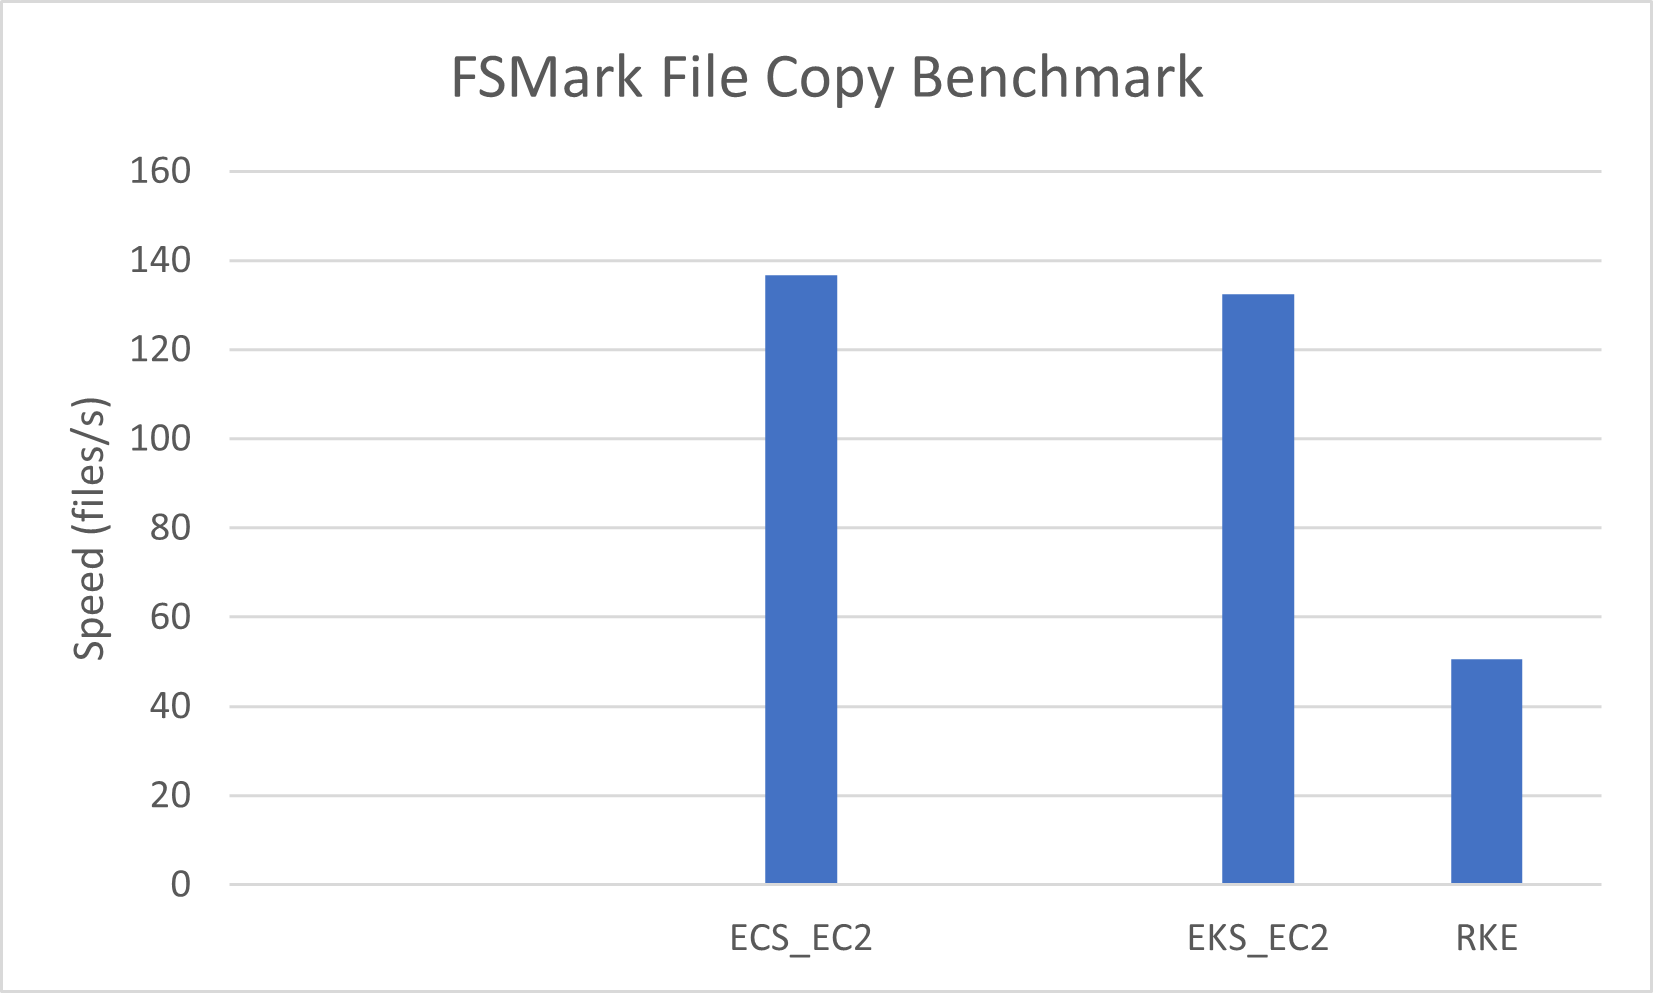
\includegraphics[width=\textwidth]{images/perf-FSMark.png}
  \caption{\emph{Performance}: Average maximum speed achieved whilst completing the fs\_mark Benchmark --- higher is better}
  \label{fig:perf_FSMark}
\end{figure}

\noindent \newline It should be noted that due to file-system mount limitations, neither of the \textit{Serverless} backed instances (that is \textit{Lambda} and \textit{fargate}) were able to complete these I\/O specific benchmarks.

\subsubsection{General Workloads}
In addition to focused hardware specific benchmarks (which are not often illustrative of real-world performance),
the following benchmarks were run to simulate performance under daily-tasks.

\paragraph{m-queens}
m-queens solves the \emph{n-queens} problem using multi-threading, measured in terms of time-to-completion (s).

Figure \ref{fig:perf_mQueens} shows the baseline \textit{RKE} cluster complete in the quickest amount of time,
followed by the \textit{EC2} backed \textit{EKS} instance almost 50\% slower.
The other instances completed this task an order of magnitude slower, all completing close to 99\% slower than baseline.

\begin{figure}[htbp]
  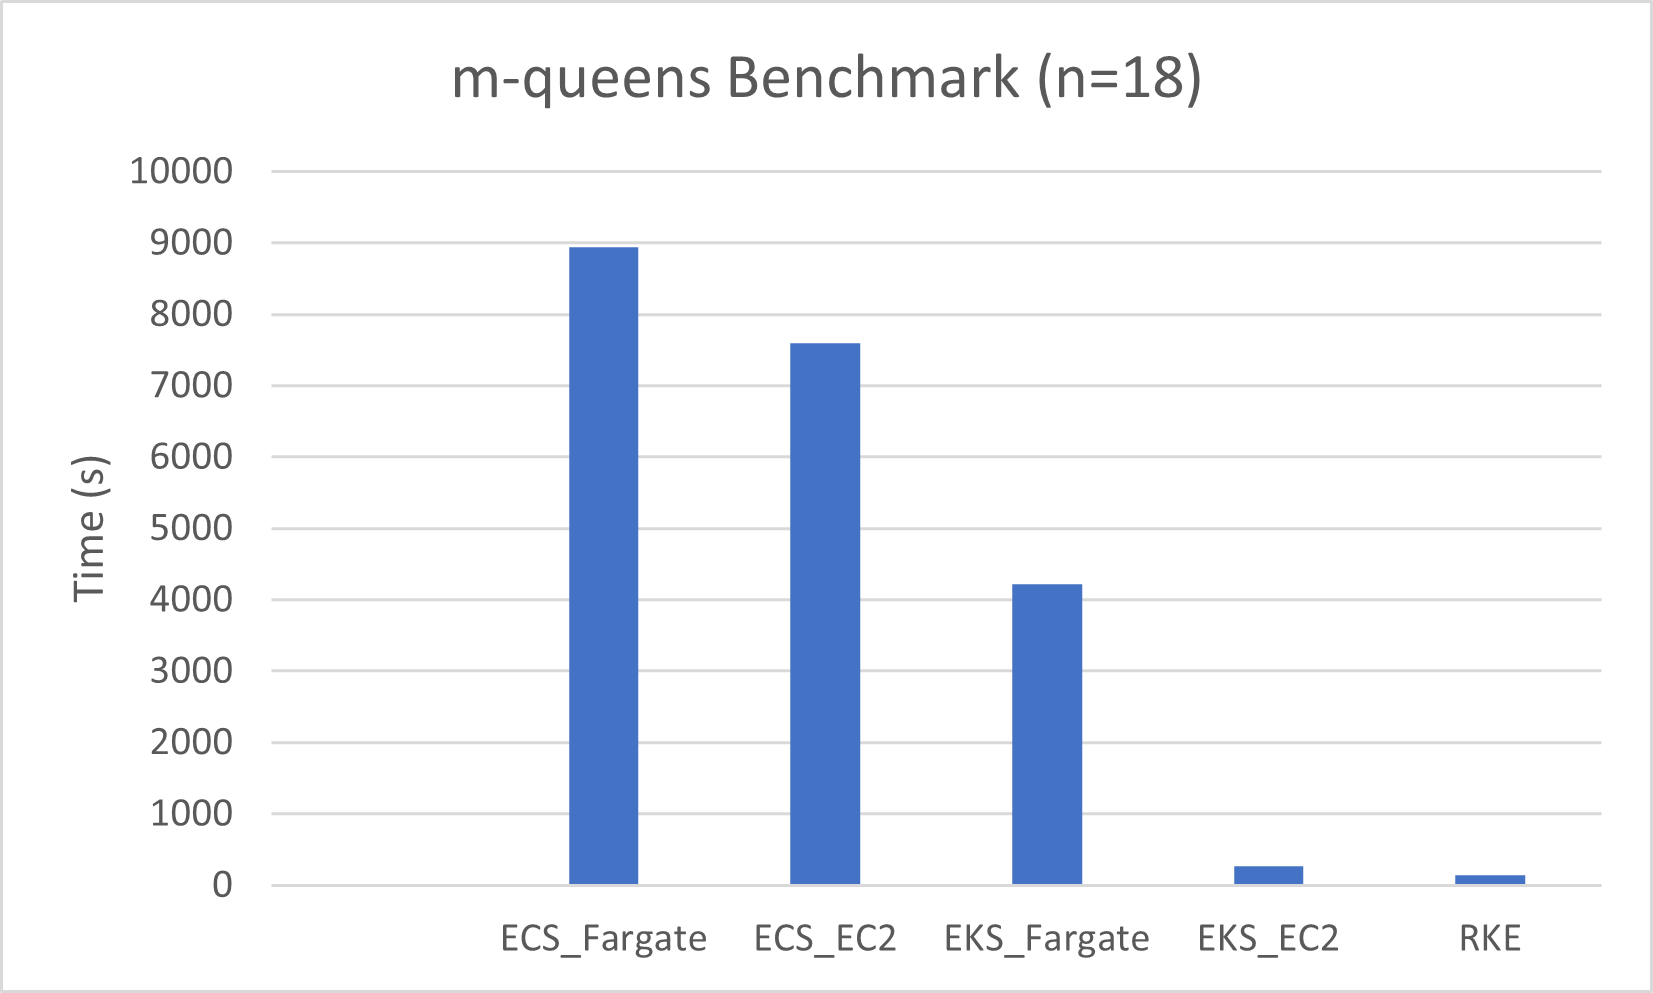
\includegraphics[width=\textwidth]{images/perf-m_queens.png}
  \caption{\emph{Performance}: Average amount of time required to solve the n-queens problem (n=18) --- lower is better}
  \label{fig:perf_mQueens}
\end{figure}

\paragraph{tool-container-benchmark}
\emph{tool-container-benchmark} simulates a general \textit{CRUD} based workload at load, measured in terms of time-to-completion (m).

Due to extreme network latency in terms of the database, the set of benchmarks were run twice,
first against an on-premise database, and the second against a cloud-hosted \textit{RDS} instance (illustrated by Figure \ref{fig:perf_tcb_default}).
Additionally in an attempt to cater for \textit{Lambda}, the set of benchmarks were re-run with a limit of 30000 \emph{events},
against both the on-premise and RDS databases
(illustrated by Figure \ref{fig:perf_tcb_30000}).

The \textit{RDS} series in Figure \ref{fig:perf_tcb_default} illustrates the \textit{EC2} backed \textit{EKS} instance performing the quickest,
followed by the two \textit{ECS} instances, with the \textit{fargate} backed and \textit{EC2} instances completing 9\% and 14\% slower respectively.
Finally, the \textit{fargate} backed \textit{EKS} instance completed the slowest (excluding the baseline \textit{RKE} instance).

The \textit{RDS} series in Figure \ref{fig:perf_tcb_30000} illustrates an anomaly with the \textit{fargate} backed \textit{ECS}
instance completing around 40\% quicker than the other instances, with all other instances completing within 30s of each other
except for \textit{Lambda} which completed close to 64\% slower.

\begin{figure}[htbp]
  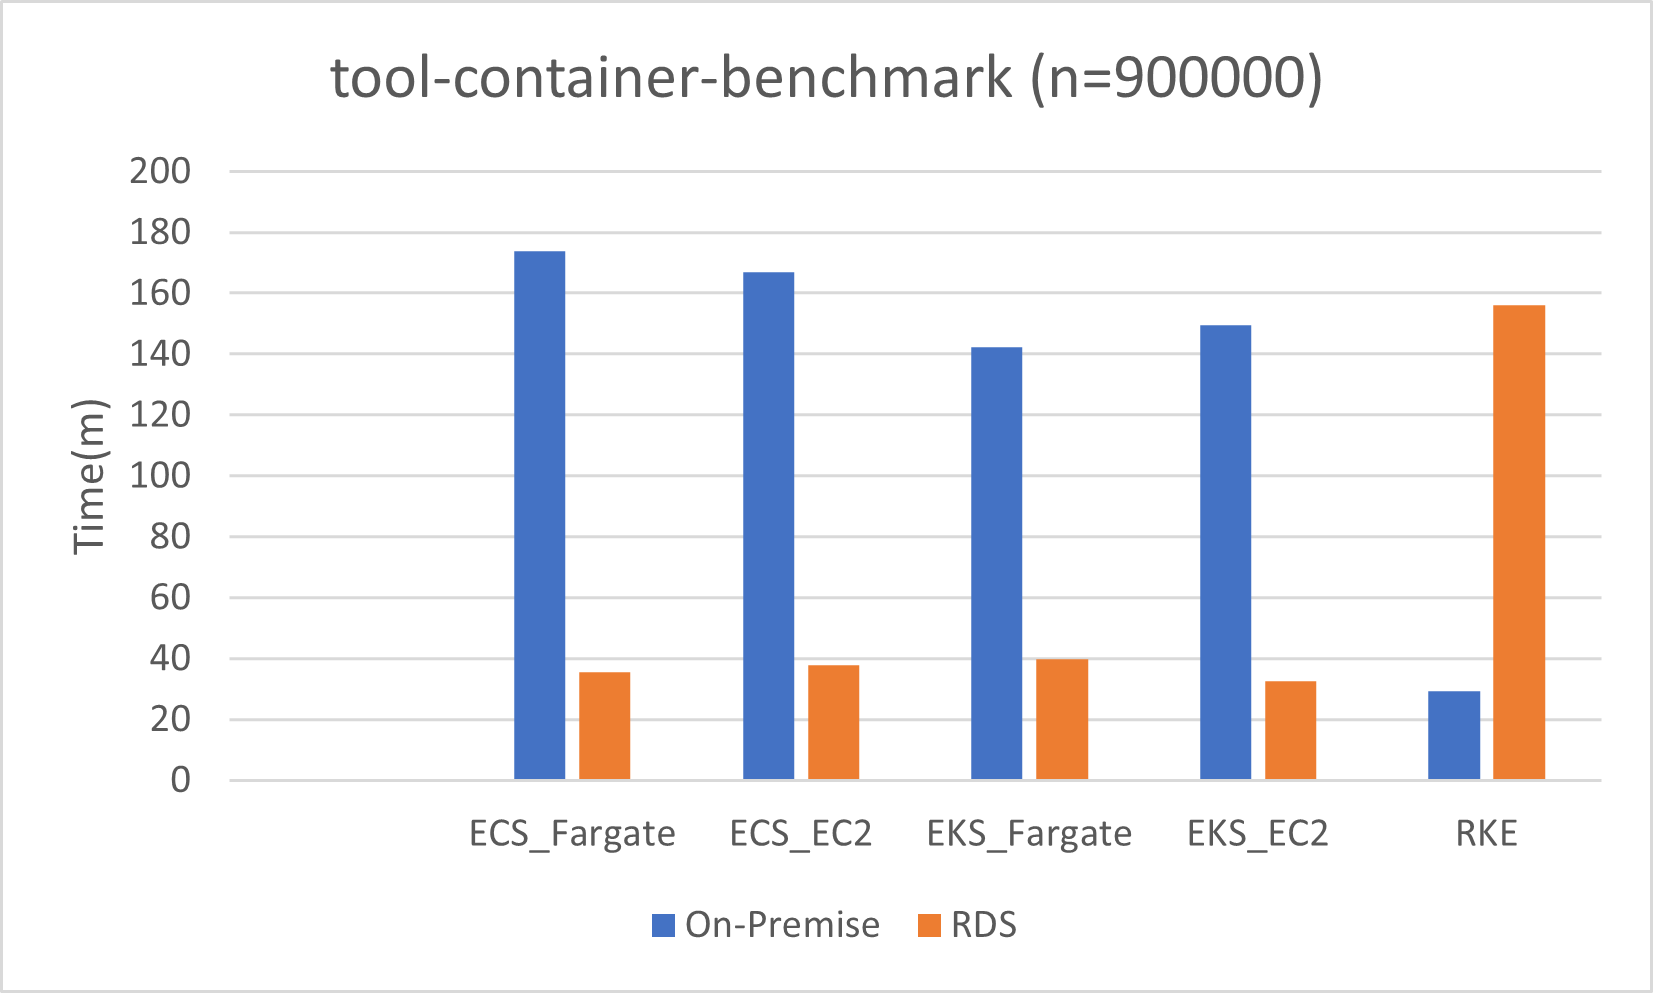
\includegraphics[width=\textwidth]{images/perf-tcb_default.png}
  \caption{\emph{Performance}: Average amount of time required to complete tool-container-benchmark (number\_of\_events=9000000) --- lower is better}
  \label{fig:perf_tcb_default}
\end{figure}

\begin{figure}[htbp]
  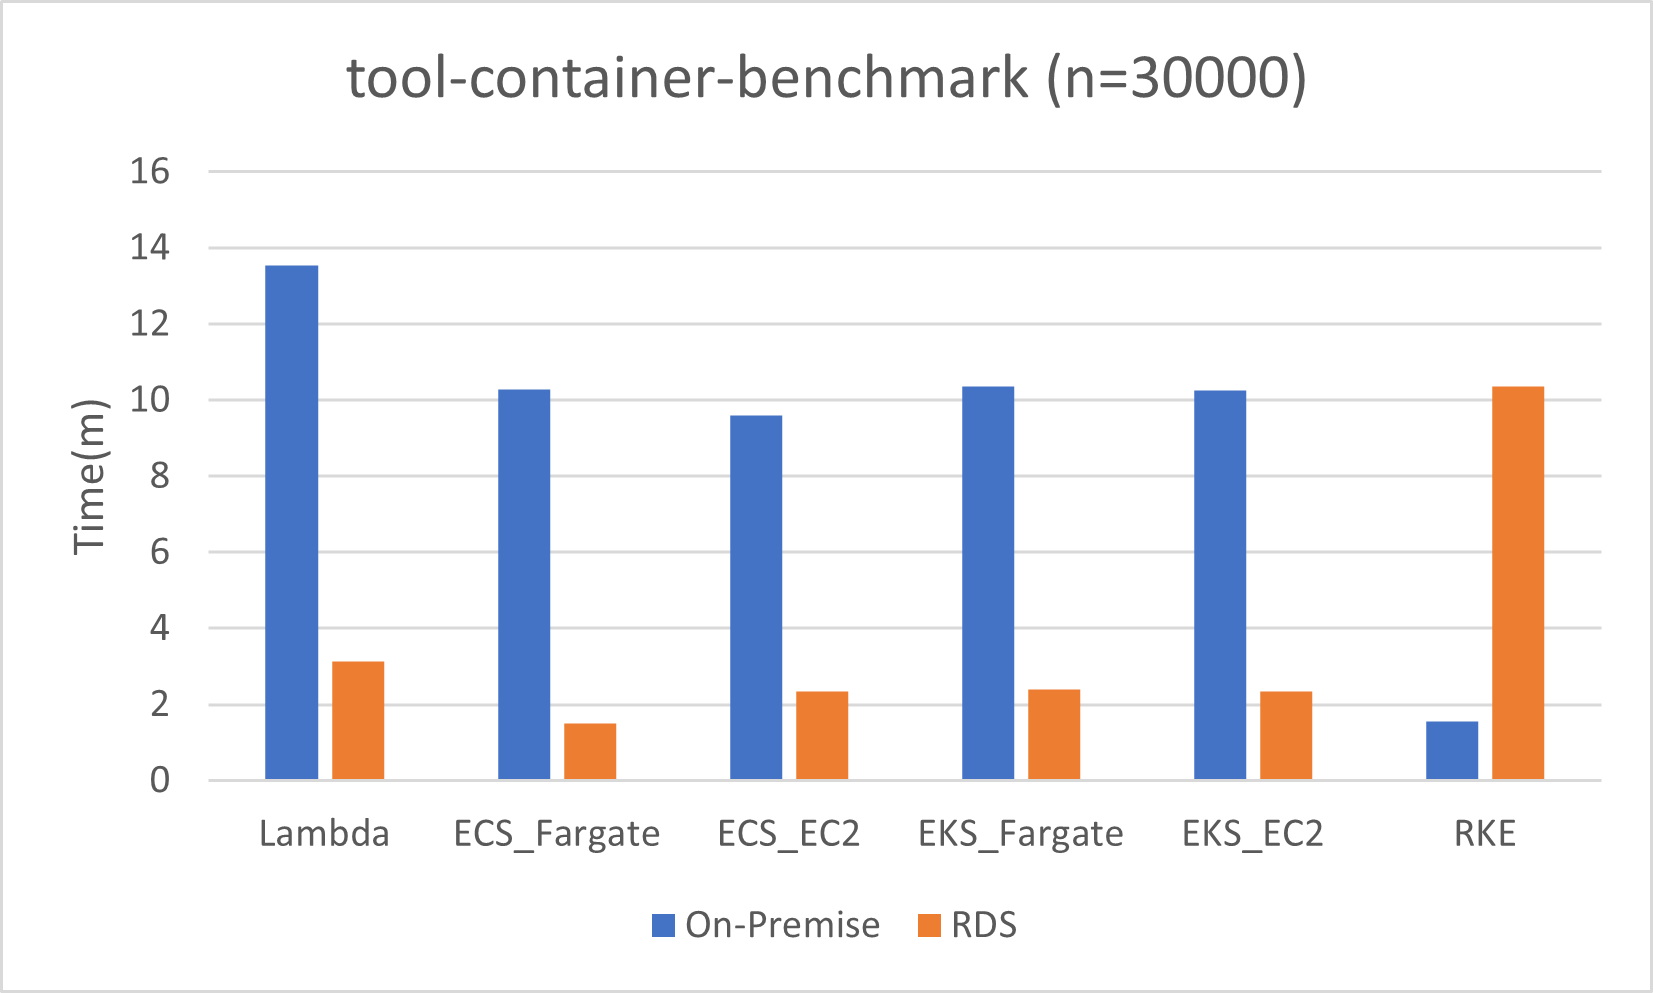
\includegraphics[width=\textwidth]{images/perf-tcb_30000.png}
  \caption{\emph{Performance}:Average amount of time required to complete tool-container-benchmark (number\_of\_events=30000) --- lower is better}
  \label{fig:perf_tcb_30000}
\end{figure}

\begin{figure}[htbp]
  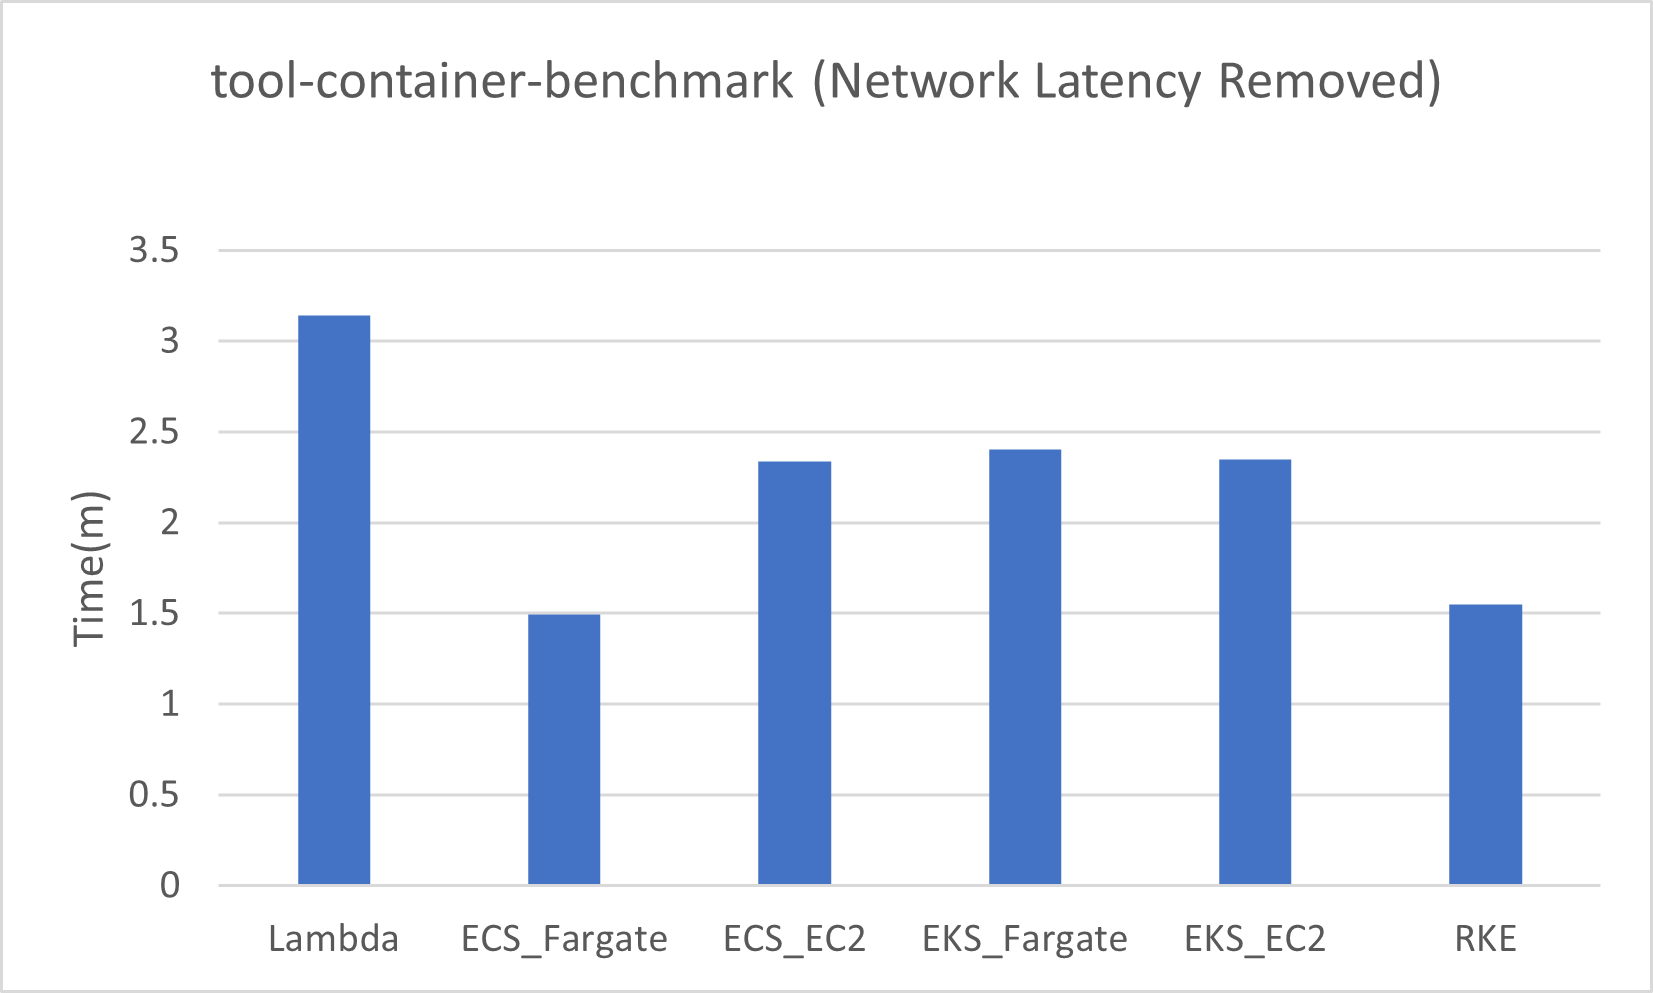
\includegraphics[width=\textwidth]{images/perf-tcb_network.png}
  \caption{\emph{Performance}:Average amount of time required to complete tool-container-benchmark, measured against Database closest to instance 
  (number\_of\_events=30000) --- lower is better}
  \label{fig:perf_tcb_network}
\end{figure}

Even with the extreme network latency caused by the database, a clear performance difference is seen by the \textit{on-premise} series in both Figures\ref{fig:perf_tcb_default} and Figures\ref{fig:perf_tcb_30000}
when comparing between the various instances (excluding the baseline instance).

Figure \ref{fig:perf_tcb_network} compares the results of each instance with the database located closest to it (in an effort to remove network latency as a factor of comparison) with \textit{number-of-events} set to 30000,
which continues to illustrate the pattern of \textit{EKS} performing better than \textit{ECS},
and \textit{EC2} backed instances performing better than their \textit{fargate} backed instances.


\subsection{Cost}
Figure\ref{fig:cost_workload} illustrates the difference in average costing when running \emph{tool-container-benchmark} three times with 30000 events against an \textit{RDS} instance, measured in US Dollars.
This table includes the dollar costing of running the actual workload (for the given period) and the cost of all dependencies,
this may include the environment or required additional services like an \textit{ALB}, over a given period.
The \textit{Serverless} instances have the advantage with \textit{Lambda} costing the lowest amount, followed by the \textit{fargate} backed \textit{ECS} and \textit{EKS} instances.
The two \textit{EC2} instances follow with \textit{ECS} and \textit{EKS} respectively.

Table\ref{fig:cost_projected} projects the costing of running a long-lived services on each platform. Here we see the two \textit{ECS} backed instances taking the lead,
with two \textit{EKS} backed instances following. For both of the above results, when scaling the cost of an \textit{EC2} instance to a cost per container
(as a single \textit{VM} can run 32 containers of the tested spec at the same cost), \textit{fargate} begins to exceed the cost of \textit{EC2}.
Additionally the \textit{EKS} platform cost is per cluster (not per container workload), therefore the additional \$73 cost per month of \textit{EKS} needs to be seen in the context of the amount of workloads being run on a cluster.
It should be noted that due to \textit{Lambda}'s time-limitation of 15 minutes, the value in this table is a theoretical project based on cost per second.

\begin{figure}[htbp]
  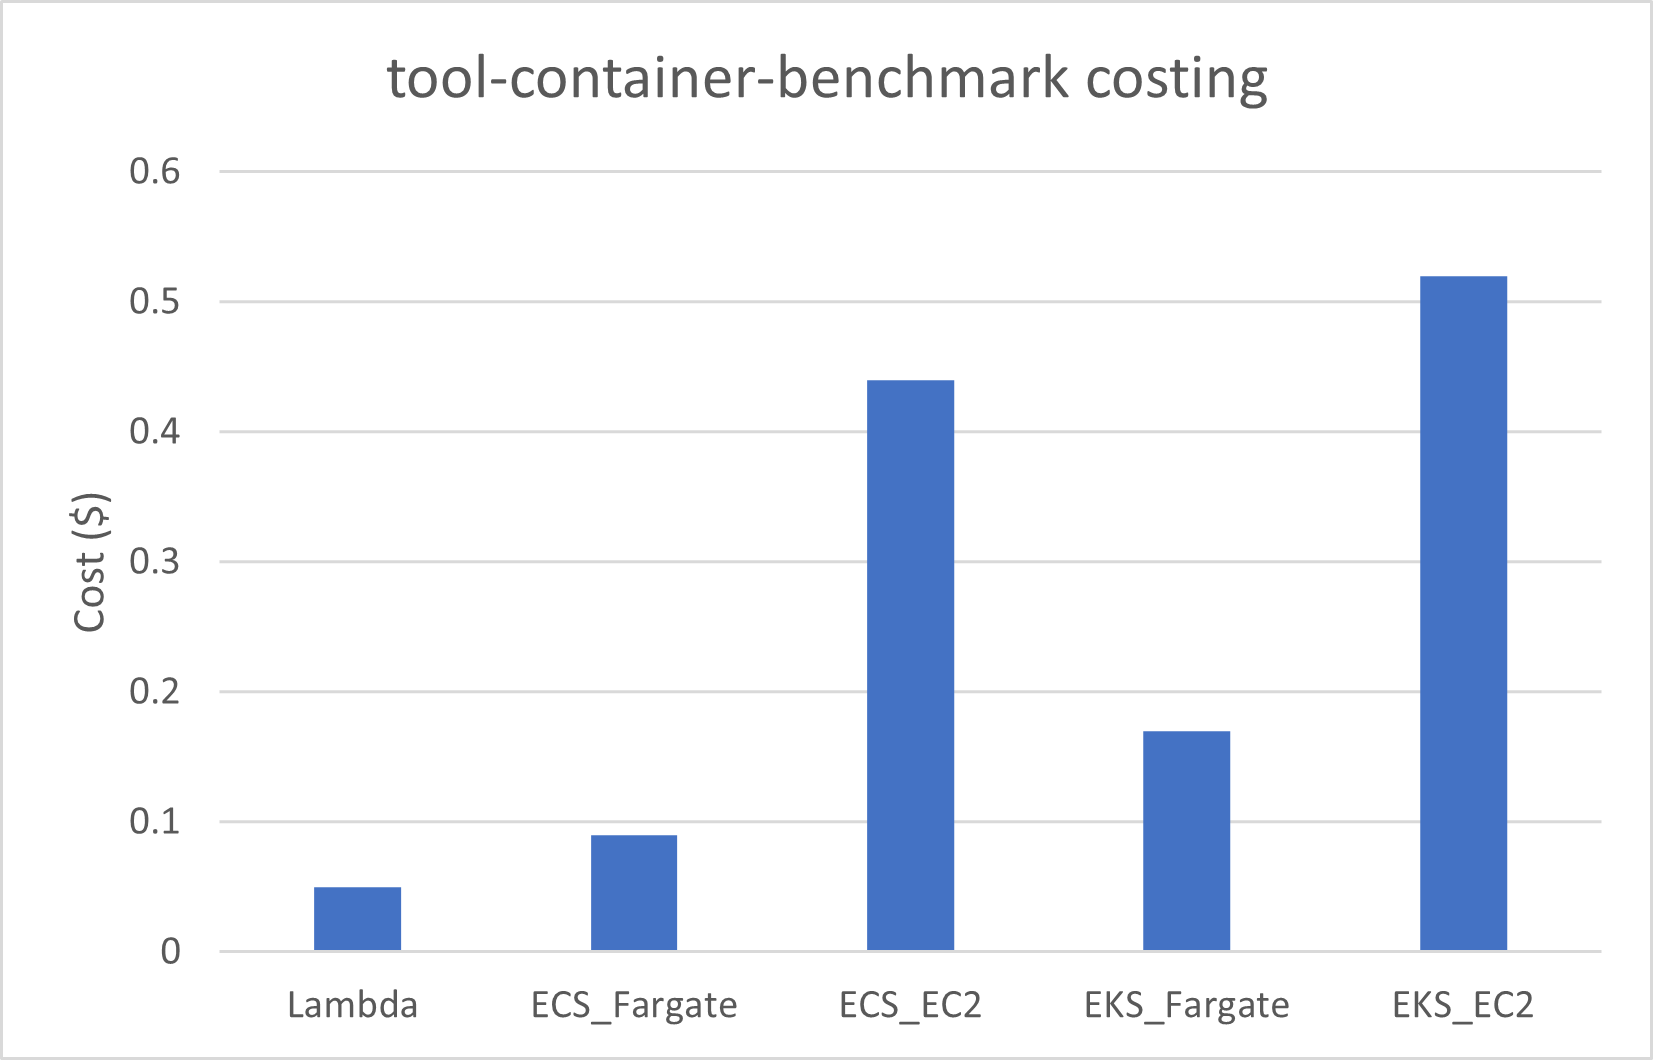
\includegraphics[width=\textwidth]{images/cost-workload.png}
  \caption{\emph{Cost}: Average cost of running \emph{tool-container-benchmark} with 30000 events --- lower is better}
  \label{fig:cost_workload}
\end{figure}

\begin{table}[htbp]
  \caption{\emph{Cost}: Projected costing (\$) of running a sample long-lived service per solution for a month and year}
  \small
  \begin{tabularx}{1\textwidth}{X | X | X }
    \space            & \bf{Monthly} & \bf{Annually} \\
    \hline
    \bf{Lambda      } & 120.11       & 1441.32       \\
    \bf{ECS\_Fargate} & 40.99        & 491.88        \\
    \bf{ECS\_EC2    } & 40.623125    & 487.4775      \\
    \bf{EKS\_Fargate} & 113.99       & 1367.88       \\
    \bf{EKS\_EC2    } & 113.623125   & 1363.4775     \\
  \end{tabularx}
  \label{fig:cost_projected}
\end{table}


\subsection{Resilience and Reliability}
Each platform was subjected to \textit{Chaos-Engineering} style tests to assert a level of resilience and reliability under extreme circumstances.

Figure\ref{fig:rr_scaling} illustrates the average amount of \textit{downtime} when scaling down the number of container-workloads to 0 and back to 1, measured in seconds.
The two \textit{EC2} backed workloads completed the scaling in the quickest, with \textit{EKS} completing first, followed by \textit{ECS}.
The two \textit{fargate} workloads followed, with \textit{ECS} completing 33\% quicker than \textit{EKS}.
It should be noted that due to inability to scale \textit{Lamda} functions, it did not participate in this test.

Figure\ref{fig:rr_deleteContainer} illustrates the average amount of time taken between a container workload being forcibly killed, and the workload being restarted, and ready to respond.
\textit{EKS} once again responded to this 35\% quicker than the \textit{ECS} workload, where the controller still noted the removed container as active and ready.
It should be noted that due to the \textit{Serverless} nature of both \textit{Lambda} and \textit{fargate}, neither of these participated in this test.

Figure\ref{fig:rr_reboot} illustrates the average amount of time taken between an underlying host being rebooted unexpectedly, the workload being restarted, and ready to respond.
\textit{ECS} handled the scale-in process 17\% faster than its \textit{EKS} counter-part.
It should be noted that due to the \textit{Serverless} nature of both \textit{Lambda} and \textit{fargate}, neither of these participated in this test.

\begin{figure}[htbp]
  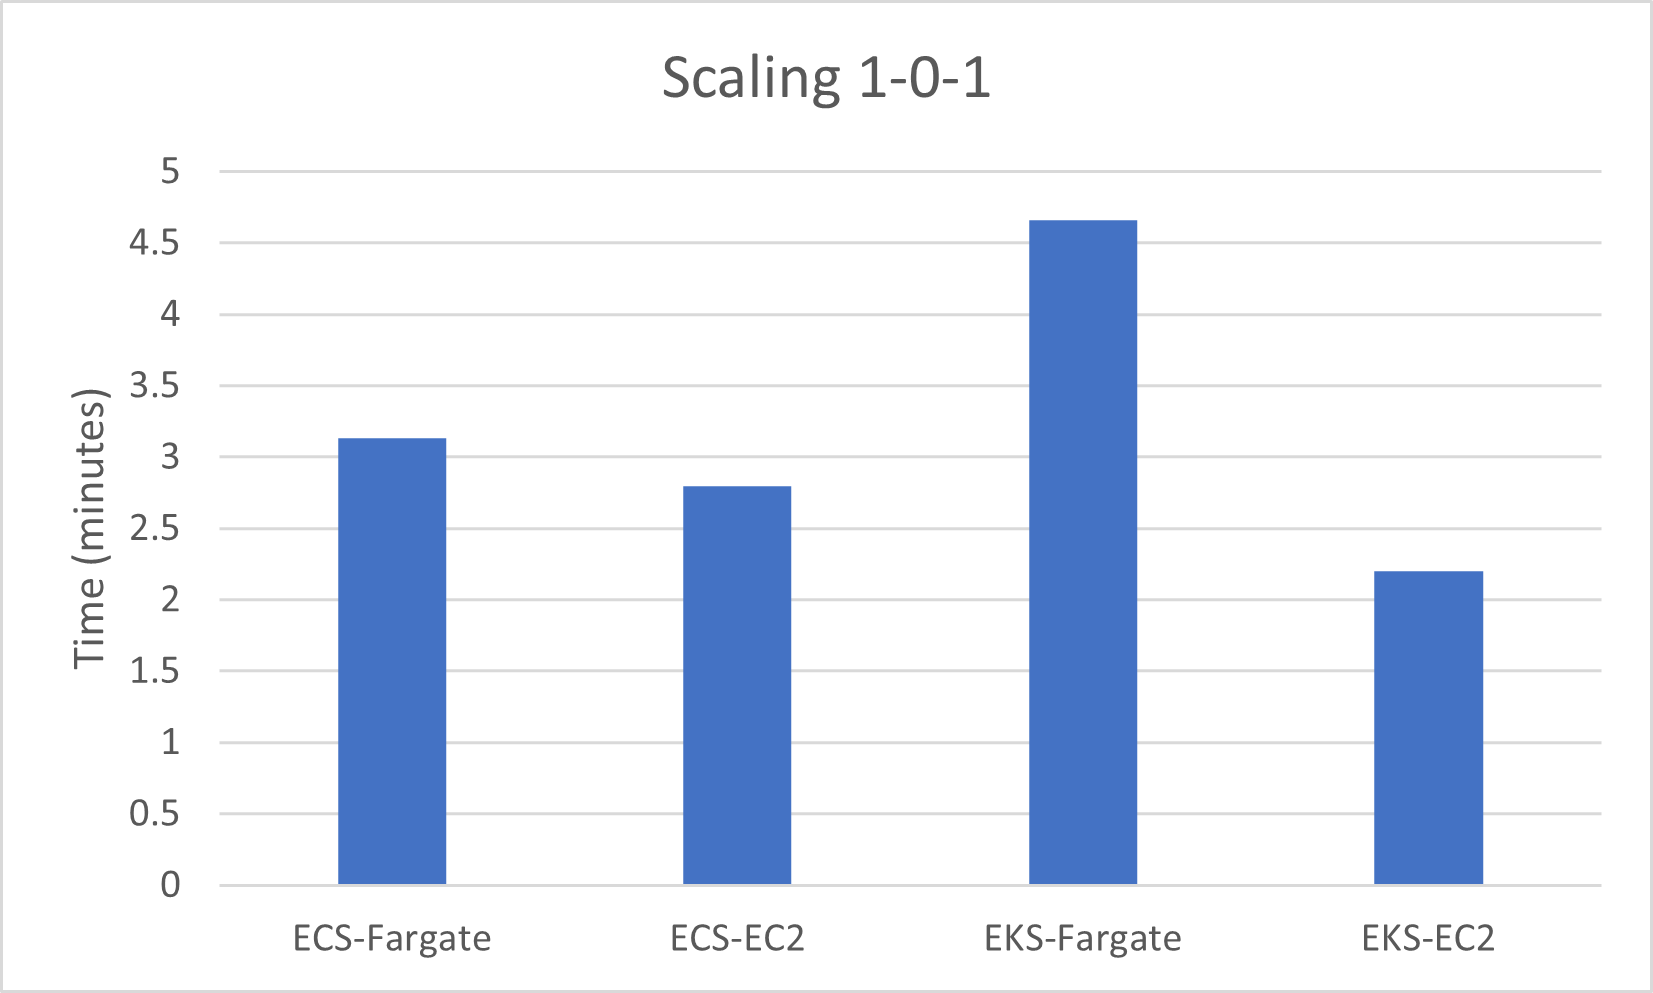
\includegraphics[width=\textwidth]{images/rr-scaling.png}
  \caption{\emph{Resilience and Reliability}: Average amount of downtime measured between scaling operations from one instance, to no instances, and back to one instance --- lower is better}
  \label{fig:rr_scaling}
\end{figure}

\begin{figure}[htbp]
  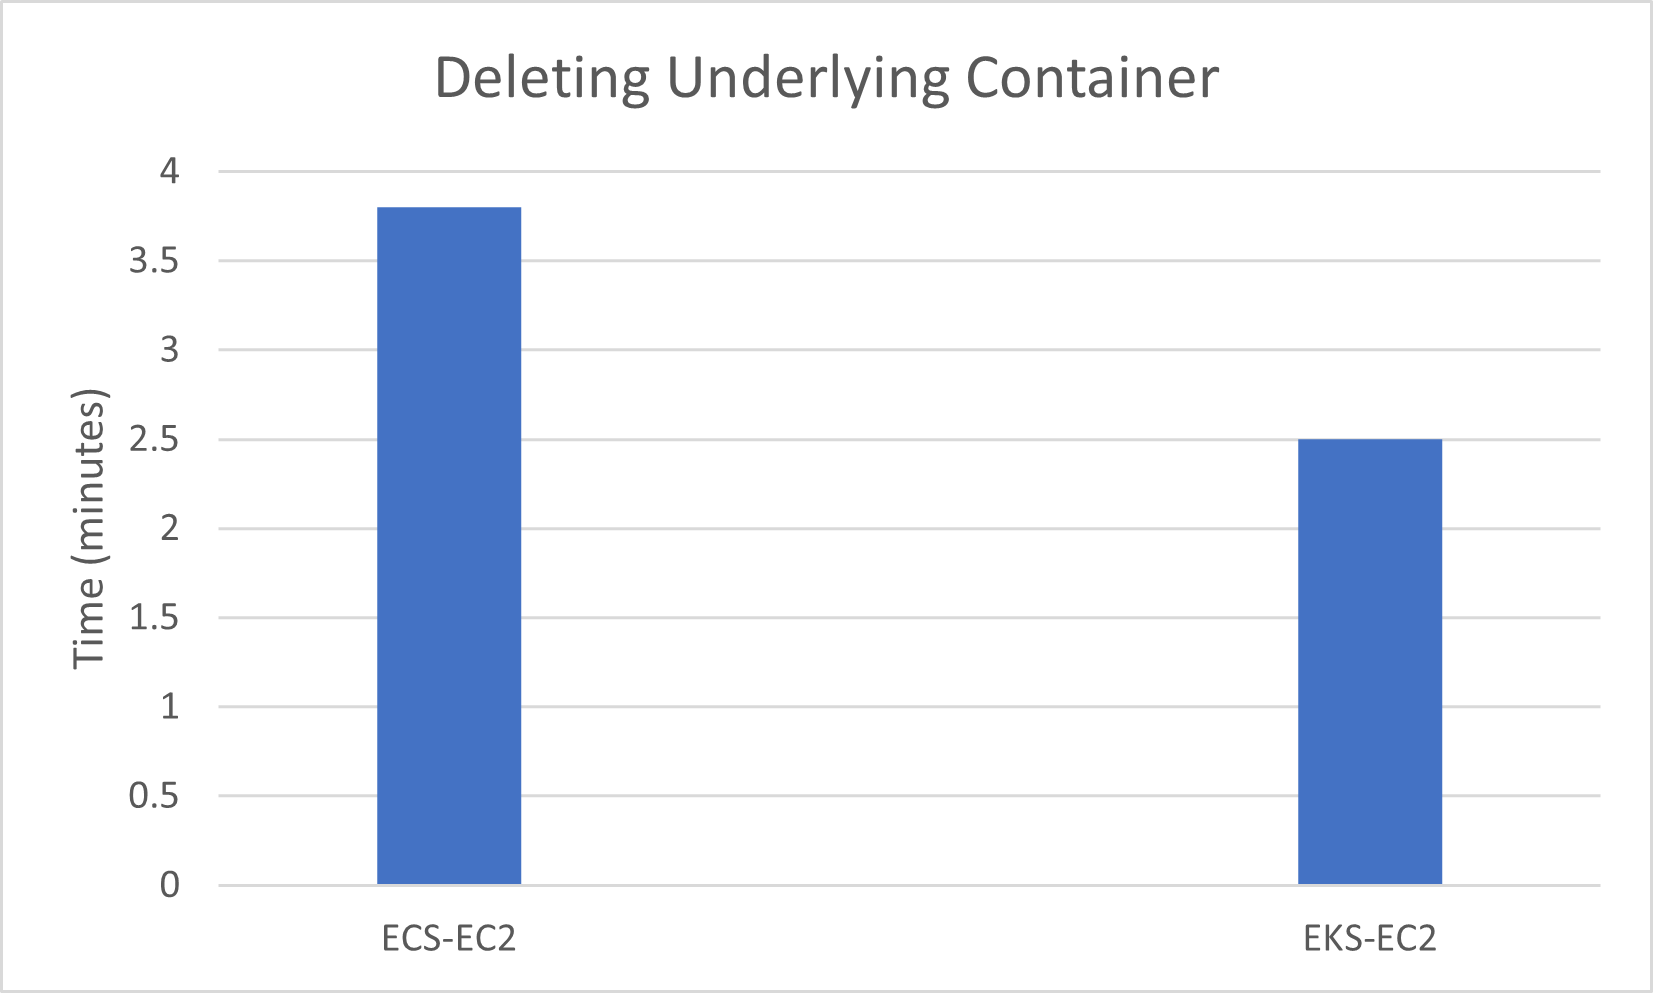
\includegraphics[width=\textwidth]{images/rr-deleteContainer.png}
  \caption{\emph{Resilience and Reliability}: Average amount of downtime measured between deleting a container on underlying host and creation of new container instance --- lower is better}
  \label{fig:rr_deleteContainer}
\end{figure}

\begin{figure}[htbp]
  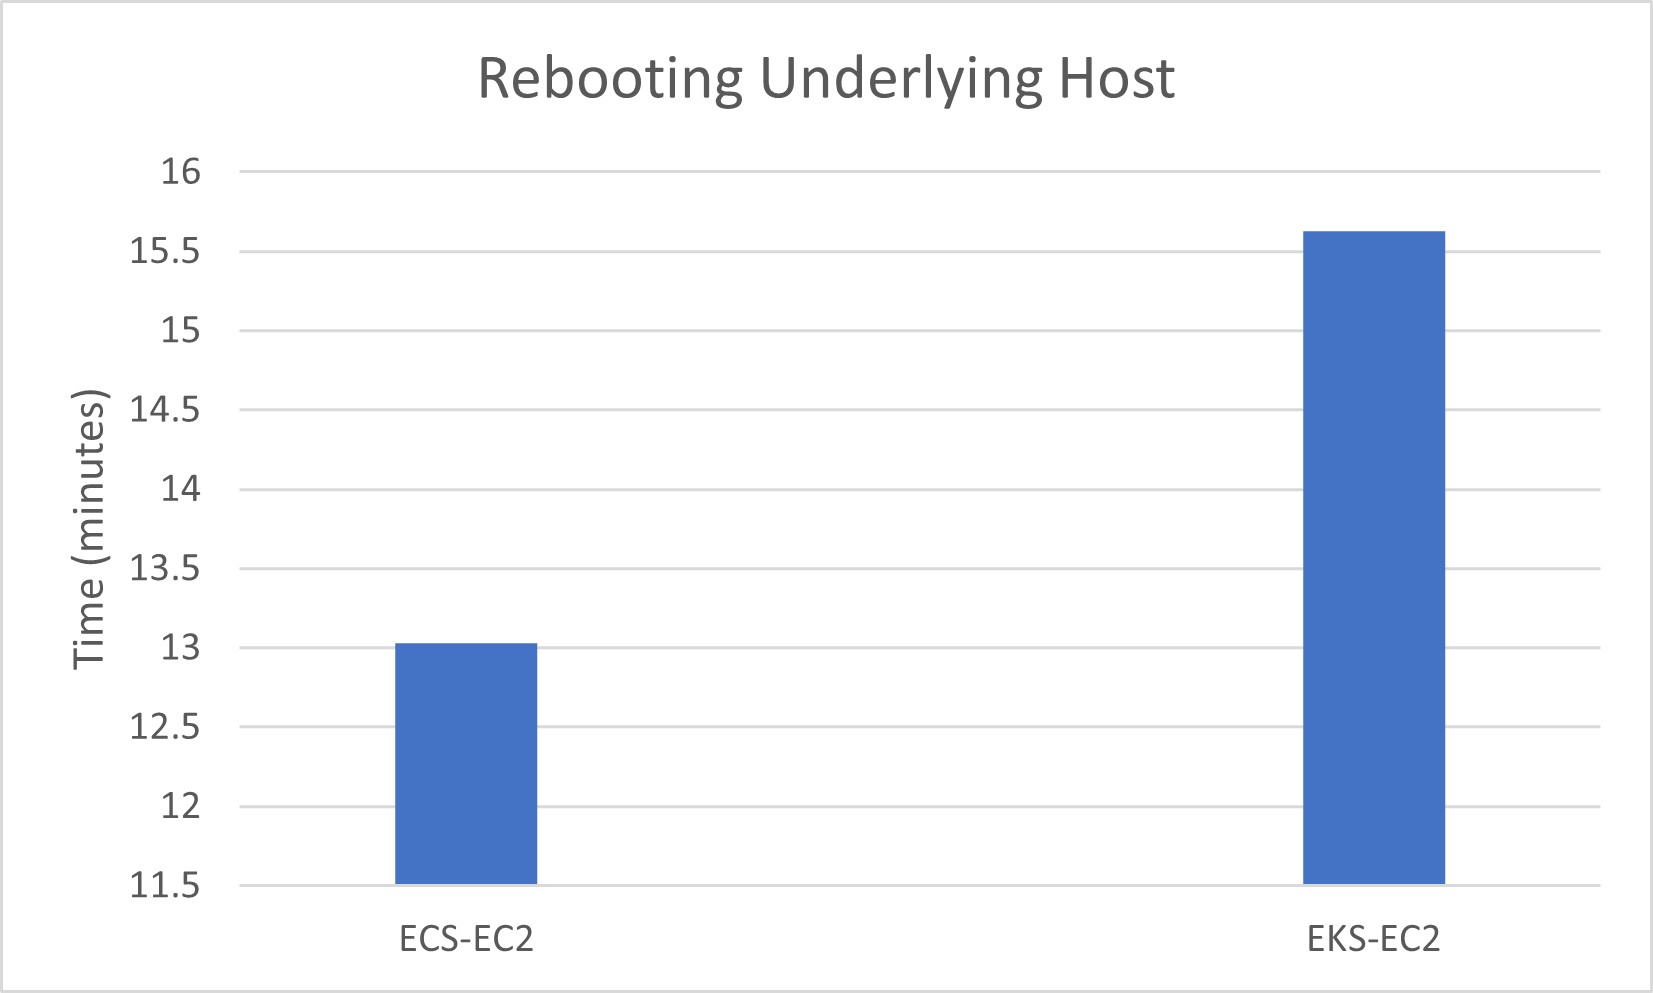
\includegraphics[width=\textwidth]{images/rr-reboot.png}
  \caption{\emph{Resilience and Reliability}: Average amount of downtime measured between deleting a container on underlying host and creation of new container instance --- lower is better}
  \label{fig:rr_reboot}
\end{figure}


\subsection{Ease-of-Use}
Each platform chosen required an architectural design, object configuration, and environment deployment.
In addition, once every environment was ready, a deployment process needed to be designed to run our test workloads on the selected platforms.

\subsubsection{Lambda}
\textit{Lambda} proved to be the easiest environment to get configured, as there was no real environment to create. Being a serverless function,
to run, it required that a Docker image exist (at this moment restricted to \textit{ECR} repositories only with a max image size of 10GB), environment variables to exist and be configured, max amount of memory
and a maximum timeout (being less than 15 minutes). This however, came at an extreme cost of flexibility and configuration.
\textit{Lambdas} being serverless \emph{functions} meant that the expected workload was a function (that is to perform a single task quickly which accepted a specific payload and response),
meant that most of the selected benchmarks were incompatible with the underlying architecture (due to the max size of 10GB of ephemeral storage available).
Where it was possible to run, the code had to be altered significantly and cater for specific \textit{Lambda} requirements.

Deployments of workloads occur via the AWS API (using the CLI, Web-Console or other tools like Terraform)

\subsubsection{ECS}
\textit{ECS} being a cloud-native \textit{orchestration} proved fairly simple to create and configure.
A \emph{cluster} needed to be created (which simply required a unique name), with \textit{capacity-providers} being registered to the cluster,
which can be of type \textit{fargate} or \textit{EC2}.
This process occurs almost immediately, and workloads can be scheduled once a providers is registered.
Workloads are defined using a \textit{task-definition}, a JSON file which describes the intended container-workloads.
Ingress connectivity would be allowed via an external \textit{ALB} which plugs directly into the rest of the architecture.

Running workloads on \textit{fargate}, being \textit{serverless} took little to no effort, as no additional resources needed to be created or configured.
Running workloads on \textit{EC2}, required far more effort, as \textit{AMI}'s needed to be built with the required \textit{ECS} agent (and dependencies) installed, tested,
and configured. Additionally \textit{ASG}'s needed to be configured and registered with the \textit{ECS} cluster before workloads would be scheduled.

Deployments of workloads occur via the AWS API (using the CLI, Web-Console or other tools like Terraform)

\subsubsection{EKS}
A bare \textit{EKS} required a similar amount of effort to create, configure as \textit{ECS}. A \emph{cluster} is created with basic configuration requirements,
further add-ons are then installed separately to add additional features required to get a \textit{k8s} cluster working in the cloud environment.
This process can take up to 30 minutes to complete.
\textit{Worker} instances are then registered to the \textit{EKS} cluster (either \textit{EC2} or \textit{fargate}).
Workloads are defined using using standard \textit{k8s} YAML object files (depending on the object type desired).
For users unfamiliar with the \textit{k8s} architecture, this can be a source of great complexity and new tooling requirements.
Ingress connectivity requires an additional ingress-controller component to be deployed into the cluster, coupled with an \textit{ALB}.

Running workloads on \textit{fargate} and \textit{EC2} is quite similar in complexity to \textit{ECS}.

Deployments of workloads occur via a specific AWS tool called \emph{eksctl}\cite{weaveworks} or the standard \textit{k8s} deployment tool \emph{kubectl}\cite{kubectl}

Figure\ref{fig:eou} illustrates the amount of time taken to bootstrap and configure each platform to be ready to run workloads (measured in minutes).
and the amount of time required to convert an existing container workload to run on each platform (measured in minutes).

\begin{figure}[htbp]
  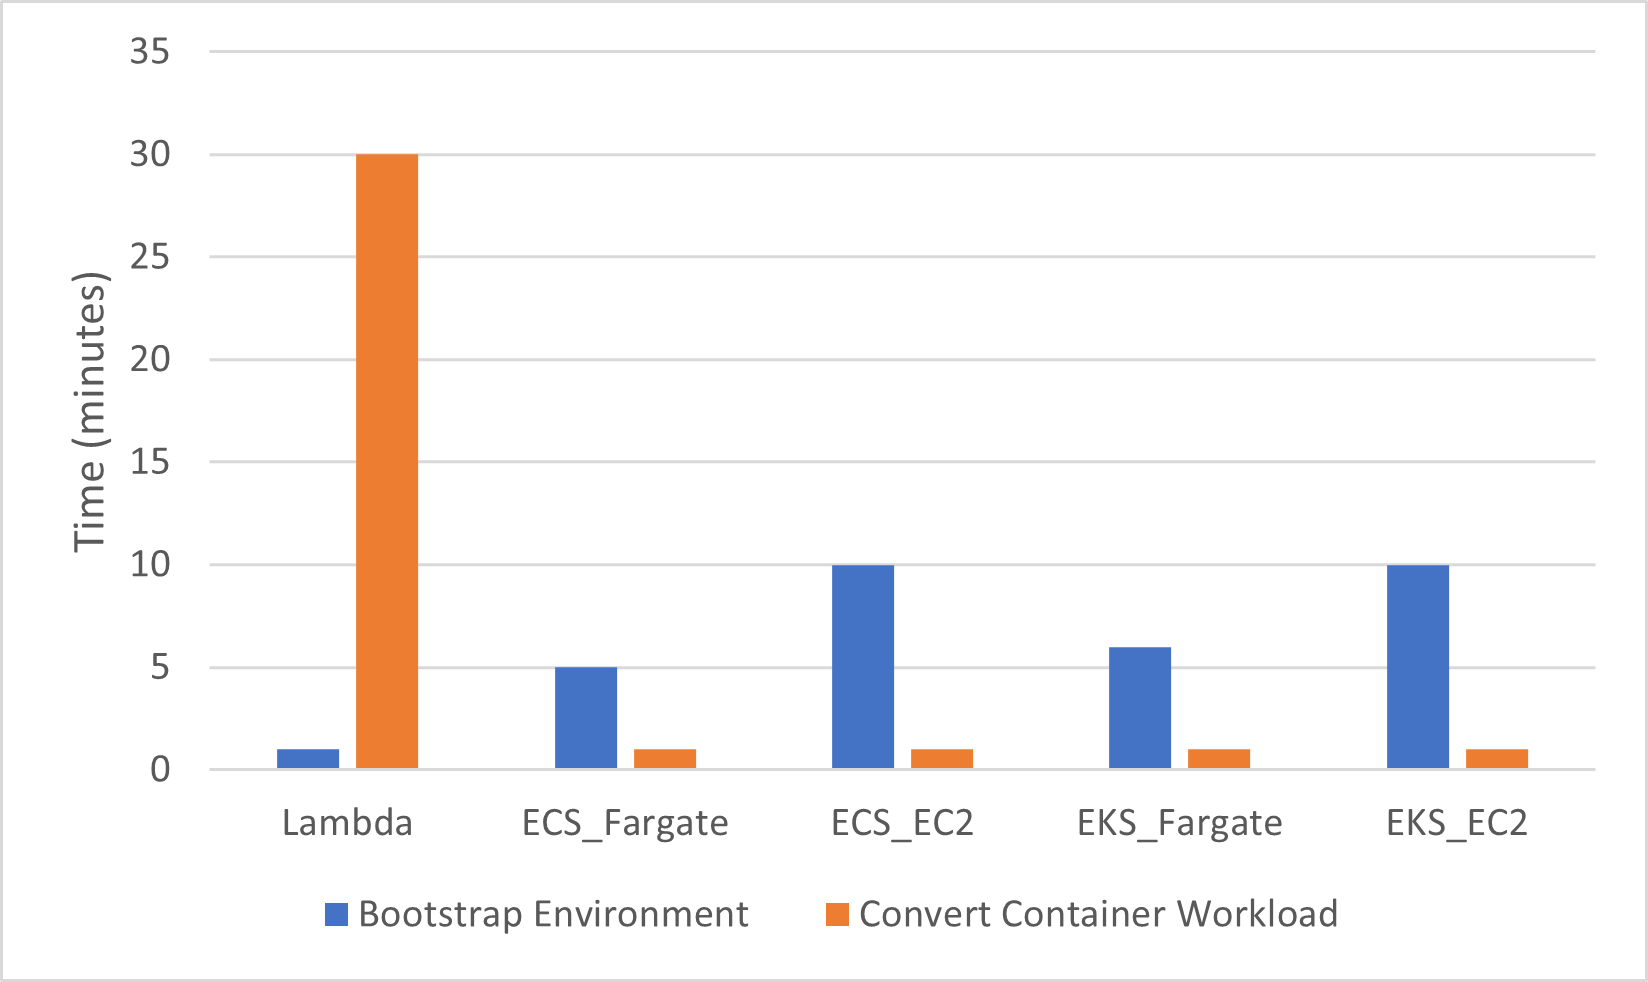
\includegraphics[width=\textwidth]{images/eou.png}
  \caption{\emph{Ease-of-Use}: Amount of time taken to complete environmental bootstrap and convert an existing container workload to run on solution --- lower is better}
  \label{fig:eou}
\end{figure}
